\section{Servidor}

É de notar que até este ponto no relatório se faz referência ao servidor como uma componente.
Nesta secção o servidor é analisado como o conjunto das suas componentes.
Descreve-se as funcionalidades de cada componente, meios de comunicação e protocolo.

\subsection{Arquitectura}

O servidor é composto por brokers e uma base de dados. Os brokers são instâncias de uma aplicação desenvolvida em Ruby, idênticos entre si, e a base de dados é PostgreSQL. A ideia é que seja indiferente o broker ao qual um cliente se liga uma vez que o comportamento é distribuído pelos restantes.
Por exemplo: dois clientes subescreverem o mesmo canal em brokers diferentes e um terceiro cliente envia uma mensagem para esse canal, então ambos os novos clientes recebem a mensagem.

\begin{figure}[H]
\centering
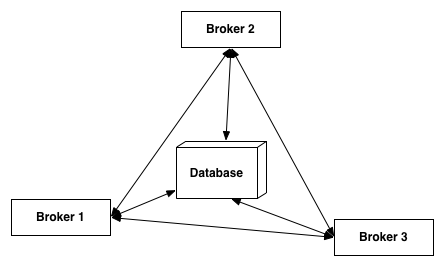
\includegraphics[width=0.65\textwidth]{brokers.png}
\caption{\textit{Visão simplista da arquitectura do servidor.}}
\label{fig:brokers-arq}
\end{figure}

Como se pode ver na figura~\ref{fig:brokers-arq} os brokers estão todos ligados entre si e cada um está ligado à base de dados. A base de dados é responsável por armazenar as mensagens persistentes, manter uma sequência que forneça identificadores únicos e registar os endereços dos servidores activos. Todas as restantes acções são da responsabilidade dos brokers, deste modo a ligação entre todos os brokers serve dois propósitos:

\begin{enumerate}
\item \textbf{Difundir mensagens de broadcast}. As mensagens que um broker recebe são difundidas pelos restantes. Isto permite que vários clientes possam subscrever os mesmos canais quando estão ligados em brokers diferentes.
\item \textbf{Informar da actualização na lista de servidores}. Quando existe um novo broker online ou um dos brokers é identificado como inactivo o novo broker ou o broker que identificou o problema, respectivamente, actualizam a base de dados e enviam uma mensagem de actualização a todos os brokers.
\end{enumerate}

\subsection{Broker}

Os brokers do servidor são instâncias de uma aplicação desenvolvida em Ruby. Cada instância difere apenas nos endereços de ligação, um endereço para a comunicação com clientes e outro endereço para comunicação com os restantes brokers.
Cada broker executa num processo Ruby e como tal mesmo na mesma máquina se pode executar diversos brokers de forma a tirar partido de paralelismo (ver secção~\ref{sec:ruby}).
A aplicação executa numa thread código orientado a eventos (ver secção~\ref{sec:eventmachine}). A enumeração a seguir descreve, de um modo simplista, as etapas necessárias para iniciar um broker.

\subsubsection{Componentes}
Cada broker inicía dois servidores de websockets, um para comunicação com os clientes e outro para comunicação com os restantes brokers.

\hl{}

\textbf{Novo servidor}
\begin{enumerate}
\item Iniciar o servidor que recebe ligações dos restantes brokers.
\item Registar o endereço do servidor na base de dado
\item Criar a ligação a todos os brokers que estão activos na base de dados.
\item Utilizar cada ligação para informar da actualização da lista de brokers.
\item Iniciar o servidor de websockets.
\end{enumerate}



\subsection{Base de Dados}
A base de dados é responsável por armazenar as mensagens persistentes, manter uma sequência que forneça identificadores únicos e registar os endereços dos servidores activos.

Funcionalidades da base de dados:
Guardar mensagens dos canais com persistência.
Guardar endereços dos servidores.

na escrita de mensagens nos canais (permite determinar quem enviou primeiro)
na reescrita do estado dos dos servidores
na obtenção de um identificador único para um utilizador

\renewcommand*{\lstlistingname}{SQL}
\lstset{language=SQL, caption={SQL para criar a base de dados}}
\begin{lstlisting}
CREATE SEQUENCE user_id START 1;

CREATE TABLE IF NOT EXISTS sessions (
  id SERIAL PRIMARY KEY,
  name VARCHAR,
  text TEXT);

CREATE TABLE IF NOT EXISTS servers (
  id SERIAL PRIMARY KEY,
  host VARCHAR,
  active BOOLEAN);
\end{lstlisting}

\lstset{language=SQL, caption={SQL para criar a base de dados}}
\begin{lstlisting}
SELECT nextval('user\_id')
\end{lstlisting}


A base de dados é sempre uma necessidade para as mensagens de canais persistentes.
No entanto as restantes funcionalidades podiam ser substituídas.

Para a questão de adequirir um identificador único no sistema para cada cliente a solução podia passar por:
um cliente envia um pedido a todos os brokers para devolver o último identificador, o cliente recolhe todas as mensagens e utiliza o valor mais alto para gerar o próximo identificador. Esta solução teria o problema da concurrência e como tal seria necessária passar um \textit{mutex}, por exemplo, para garantir que apenas um broker pode pedir um identificador de cada vez.

Para identificar os brokers activos podia existir um monitor responsável por fornecer os endereços dos brokers activos a um novo broker e do mesmo modo identificar falhas e informar os brokers.

\subsection{Mensagens}

As mensagens que o servidor reconhecem são no seguinte formato:

[[instructions], message]

Pode resumir-se que é um array que contém uma lista de instruções na posição zero e uma mensagem na posição um. Existem os seguintes tipos de mensagens:

\begin{enumerate}
\item
\texttt{[[``subscribe''], ``channel'']}

Quando a primeira instrução é ``subscribe'' o servidor subscreve o cliente ao canal com o nome que vai no lugar da mensagem.

\item
\texttt{[[``subscribe'', ``persistent''], ``channel'']}

Se o subscribe for acompnhado de um persistent então o canal criado é persistente. Senão subscreve ao canal existente.

\item
\texttt{[[``unsubscribe''], ``channel'']}

Quando a primeira instrução é ``unsubscribe'' o servidor remove a descrição do cliente ao canal com o nome que vai no lugar da mensagem.

\item
\texttt{[[``all''], ``message'']}

Quando a primeira instrução é ``all'' a mensagem é enviada a todos os clientes do servidor (clientes de todos os brokers).

\item
\texttt{[[``channel 1'', ``channel 2''], ``message'']}

Quando a primeira instrução nao é ``all'' então todos as instruções são consideradas nomes de canais e a mensagem é distribuída por todos os clientes subscritos ao canal.

\end{enumerate}

\subsection{Ciclo de Vida de um Cliente}

\begin{figure}[H]
\centering
\includegraphics[width=0.65\textwidth]{server_client.png}
\caption{\textit{Ciclo de vida de um cliente.}}
\label{fig:server-client}
\end{figure}

A figura~\ref{fig:server-client} contém um diagrama de sequência que apresenta o básico da interação entre um cliente e o servidor (entenda-se por servidor como um broker do servidor).
Um cliente começa por establecer ligação a um dos brokers do servidor. Assim que a ligação é establecida o broker devolve um identificador único ao cliente. Esta etapa está identificada no bloco um na figura~\ref{fig:server-client}. Depois esta etapa inicial são três os cenários possíveiseservidor

\begin{itemize}
\item
\textbf{O cliente envia uma mensagem}

O cliente envia uma mensagem ao broker (etapa 2 da figura~\ref{fig:server-client}). A mensagem é devolvida ao cliente no processo de broadcast do servidor.

\item
\textbf{O servidor faz broadcast de uma mensagem}

O servidor envia uma mensagem no processo de broadcast de mensagens de outros clientes (etapa 3 da figura~\ref{fig:server-client}).

\item
\textbf{O cliente termina a ligação}

O cliente termina a ligação com o servidor (etapa 4 da figura~\ref{fig:server-client}).
\end{itemize}
